\documentclass{article}\usepackage[]{graphicx}\usepackage[]{color}
%% maxwidth is the original width if it is less than linewidth
%% otherwise use linewidth (to make sure the graphics do not exceed the margin)
\makeatletter
\def\maxwidth{ %
  \ifdim\Gin@nat@width>\linewidth
    \linewidth
  \else
    \Gin@nat@width
  \fi
}
\makeatother

\definecolor{fgcolor}{rgb}{0.345, 0.345, 0.345}
\newcommand{\hlnum}[1]{\textcolor[rgb]{0.686,0.059,0.569}{#1}}%
\newcommand{\hlstr}[1]{\textcolor[rgb]{0.192,0.494,0.8}{#1}}%
\newcommand{\hlcom}[1]{\textcolor[rgb]{0.678,0.584,0.686}{\textit{#1}}}%
\newcommand{\hlopt}[1]{\textcolor[rgb]{0,0,0}{#1}}%
\newcommand{\hlstd}[1]{\textcolor[rgb]{0.345,0.345,0.345}{#1}}%
\newcommand{\hlkwa}[1]{\textcolor[rgb]{0.161,0.373,0.58}{\textbf{#1}}}%
\newcommand{\hlkwb}[1]{\textcolor[rgb]{0.69,0.353,0.396}{#1}}%
\newcommand{\hlkwc}[1]{\textcolor[rgb]{0.333,0.667,0.333}{#1}}%
\newcommand{\hlkwd}[1]{\textcolor[rgb]{0.737,0.353,0.396}{\textbf{#1}}}%
\let\hlipl\hlkwb

\usepackage{framed}
\makeatletter
\newenvironment{kframe}{%
 \def\at@end@of@kframe{}%
 \ifinner\ifhmode%
  \def\at@end@of@kframe{\end{minipage}}%
  \begin{minipage}{\columnwidth}%
 \fi\fi%
 \def\FrameCommand##1{\hskip\@totalleftmargin \hskip-\fboxsep
 \colorbox{shadecolor}{##1}\hskip-\fboxsep
     % There is no \\@totalrightmargin, so:
     \hskip-\linewidth \hskip-\@totalleftmargin \hskip\columnwidth}%
 \MakeFramed {\advance\hsize-\width
   \@totalleftmargin\z@ \linewidth\hsize
   \@setminipage}}%
 {\par\unskip\endMakeFramed%
 \at@end@of@kframe}
\makeatother

\definecolor{shadecolor}{rgb}{.97, .97, .97}
\definecolor{messagecolor}{rgb}{0, 0, 0}
\definecolor{warningcolor}{rgb}{1, 0, 1}
\definecolor{errorcolor}{rgb}{1, 0, 0}
\newenvironment{knitrout}{}{} % an empty environment to be redefined in TeX

\usepackage{alltt}
\usepackage{natbib}
\IfFileExists{upquote.sty}{\usepackage{upquote}}{}
\begin{document}

\title{Pride and Prejudice Wordcloud}
\author{Dayana Moncada}
\maketitle

\begin{abstract}
In this article we construct a wordcloud, using the tidytext R package, for Jane Austen's Pride and Prejudice novel. This is a replica from my professor Dr. Charles Redmond's work with the Sense and Sensibility's wordcloud using the same packages. I will try to tweak and personalize some codes. Finally, this is a learning experience and comments/questions are deeply appreciated.

\end{abstract}

\textit{Pride and Prejudice} 
Pride and Prejudice is one of Austen's famous book where she tells the love story between Elizabeth Bennet and Mr. Darcy. For a lot of time, this novel has been considered a classic "must=read". Jane Austen shows us "the folly of judging by first impressions and superbly evokes the friendships, gossip and sobberies of provincial middle-class life."\footnote{Amazon.com}

\section{The Jane Austen Package} 
This package contains the complete text of Jane Austen’s 6 completed, published novels, formatted to be convenient for text analysis.

\begin{knitrout}
\definecolor{shadecolor}{rgb}{0.969, 0.969, 0.969}\color{fgcolor}\begin{kframe}
\begin{alltt}
\hlkwd{library}\hlstd{(janeaustenr)}
\hlstd{pnp}\hlkwb{<-}\hlkwd{austen_books}\hlstd{()}
\end{alltt}
\end{kframe}
\end{knitrout}

This dataframe has two columns, one for each line in Austen's novels, and one indicating which book the line is from.  Let's first filter, using dplyr, so that we have only the lines from Pride and Prejudice:

\begin{knitrout}
\definecolor{shadecolor}{rgb}{0.969, 0.969, 0.969}\color{fgcolor}\begin{kframe}
\begin{alltt}
\hlkwd{library}\hlstd{(dplyr)}
\hlstd{pnp}\hlkwb{<-}\hlstd{pnp}\hlopt
  \hlkwd{filter}\hlstd{(book} \hlopt{==} \hlstr{'Pride & Prejudice'}\hlstd{)}

\hlkwd{head}\hlstd{(prideprejudice)}
\end{alltt}
\begin{verbatim}
## [1] "PRIDE AND PREJUDICE" ""                    "By Jane Austen"     
## [4] ""                    ""                    ""
\end{verbatim}
\end{kframe}
\end{knitrout}

\noindent Now we are ready for some data cleaning.

\section{Some Data Cleaning}

We would like to remove all of the `Chapter' lines.  We can use dplyr again, along with the package stringr.

\begin{knitrout}
\definecolor{shadecolor}{rgb}{0.969, 0.969, 0.969}\color{fgcolor}\begin{kframe}
\begin{alltt}
\hlkwd{library}\hlstd{(stringr)}
\hlstd{pnp}\hlkwb{<-}\hlstd{pnp}\hlopt
  \hlkwd{filter}\hlstd{(}\hlopt{!}\hlkwd{str_detect}\hlstd{(pnp}\hlopt{$}\hlstd{text,}\hlstr{'^CHAPTER'}\hlstd{))}
\end{alltt}
\end{kframe}
\end{knitrout}

Next, we would like to remove the front matter.  By inspection, we have determined that the front matter ends on line 9.  Therefore we can redefine sns to begin on line 10:
\begin{knitrout}
\definecolor{shadecolor}{rgb}{0.969, 0.969, 0.969}\color{fgcolor}\begin{kframe}
\begin{alltt}
\hlstd{pnp}\hlkwb{<-}\hlstd{pnp[}\hlnum{10}\hlopt{:}\hlnum{12030}\hlstd{,]}
\end{alltt}
\end{kframe}
\end{knitrout}

\section{The Wordcloud}
To make the wordcloud, we first have to break up the lines into words.  We can use a function from the tidytext package for this:

\begin{knitrout}
\definecolor{shadecolor}{rgb}{0.969, 0.969, 0.969}\color{fgcolor}\begin{kframe}
\begin{alltt}
\hlkwd{library}\hlstd{(tidytext)}
\end{alltt}


{\ttfamily\noindent\color{warningcolor}{\#\# Warning: package 'tidytext' was built under R version 3.4.2}}\begin{alltt}
\hlstd{words_df}\hlkwb{<-}\hlstd{pnp}\hlopt
  \hlkwd{unnest_tokens}\hlstd{(word,text)}

\hlstd{words_df}
\end{alltt}
\begin{verbatim}
## # A tibble: 112,909 x 2
##                 book         word
##               <fctr>        <chr>
##  1 Pride & Prejudice           it
##  2 Pride & Prejudice           is
##  3 Pride & Prejudice            a
##  4 Pride & Prejudice        truth
##  5 Pride & Prejudice  universally
##  6 Pride & Prejudice acknowledged
##  7 Pride & Prejudice         that
##  8 Pride & Prejudice            a
##  9 Pride & Prejudice       single
## 10 Pride & Prejudice          man
## # ... with 112,899 more rows
\end{verbatim}
\end{kframe}
\end{knitrout}

We can remove common, unimportant words with the stop\_words data frame and some dplyr:
\begin{knitrout}
\definecolor{shadecolor}{rgb}{0.969, 0.969, 0.969}\color{fgcolor}\begin{kframe}
\begin{alltt}
\hlstd{words_df}\hlkwb{<-}\hlstd{words_df}\hlopt
  \hlkwd{filter}\hlstd{(}\hlopt{!}\hlstd{(word} \hlopt \hlstd{stop_words}\hlopt{$}\hlstd{word))}

\hlstd{words_df}
\end{alltt}
\begin{verbatim}
## # A tibble: 34,525 x 2
##                 book         word
##               <fctr>        <chr>
##  1 Pride & Prejudice        truth
##  2 Pride & Prejudice  universally
##  3 Pride & Prejudice acknowledged
##  4 Pride & Prejudice       single
##  5 Pride & Prejudice   possession
##  6 Pride & Prejudice      fortune
##  7 Pride & Prejudice         wife
##  8 Pride & Prejudice     feelings
##  9 Pride & Prejudice        views
## 10 Pride & Prejudice     entering
## # ... with 34,515 more rows
\end{verbatim}
\end{kframe}
\end{knitrout}

Now, we need to calculate the frequencies of the words in the novel.  Again, we can use standard dplyr techniques for this:
\begin{knitrout}
\definecolor{shadecolor}{rgb}{0.969, 0.969, 0.969}\color{fgcolor}\begin{kframe}
\begin{alltt}
\hlstd{word_freq}\hlkwb{<-}\hlstd{words_df}\hlopt
  \hlkwd{group_by}\hlstd{(word)}\hlopt
  \hlkwd{summarize}\hlstd{(}\hlkwc{count}\hlstd{=}\hlkwd{n}\hlstd{())}

\hlstd{word_freq}
\end{alltt}
\begin{verbatim}
## # A tibble: 5,831 x 2
##            word count
##           <chr> <int>
##  1   _accident_     1
##  2 _advantages_     1
##  3     _affect_     1
##  4        _all_     4
##  5         _am_     1
##  6     _another     1
##  7        _any_     1
##  8  _anybody's_     1
##  9 _appearance_     3
## 10        _are_     2
## # ... with 5,821 more rows
\end{verbatim}
\end{kframe}
\end{knitrout}

Finally, it's time to generate the wordcloud:
\begin{knitrout}
\definecolor{shadecolor}{rgb}{0.969, 0.969, 0.969}\color{fgcolor}\begin{kframe}
\begin{alltt}
\hlkwd{library}\hlstd{(wordcloud)}
\end{alltt}


{\ttfamily\noindent\itshape\color{messagecolor}{\#\# Loading required package: RColorBrewer}}\begin{alltt}
\hlkwd{library}\hlstd{(tm)}
\end{alltt}


{\ttfamily\noindent\itshape\color{messagecolor}{\#\# Loading required package: NLP}}\begin{alltt}
\hlkwd{wordcloud}\hlstd{(word_freq}\hlopt{$}\hlstd{word,word_freq}\hlopt{$}\hlstd{count,}\hlkwc{min.freq}\hlstd{=}\hlnum{25}\hlstd{)}
\end{alltt}
\end{kframe}
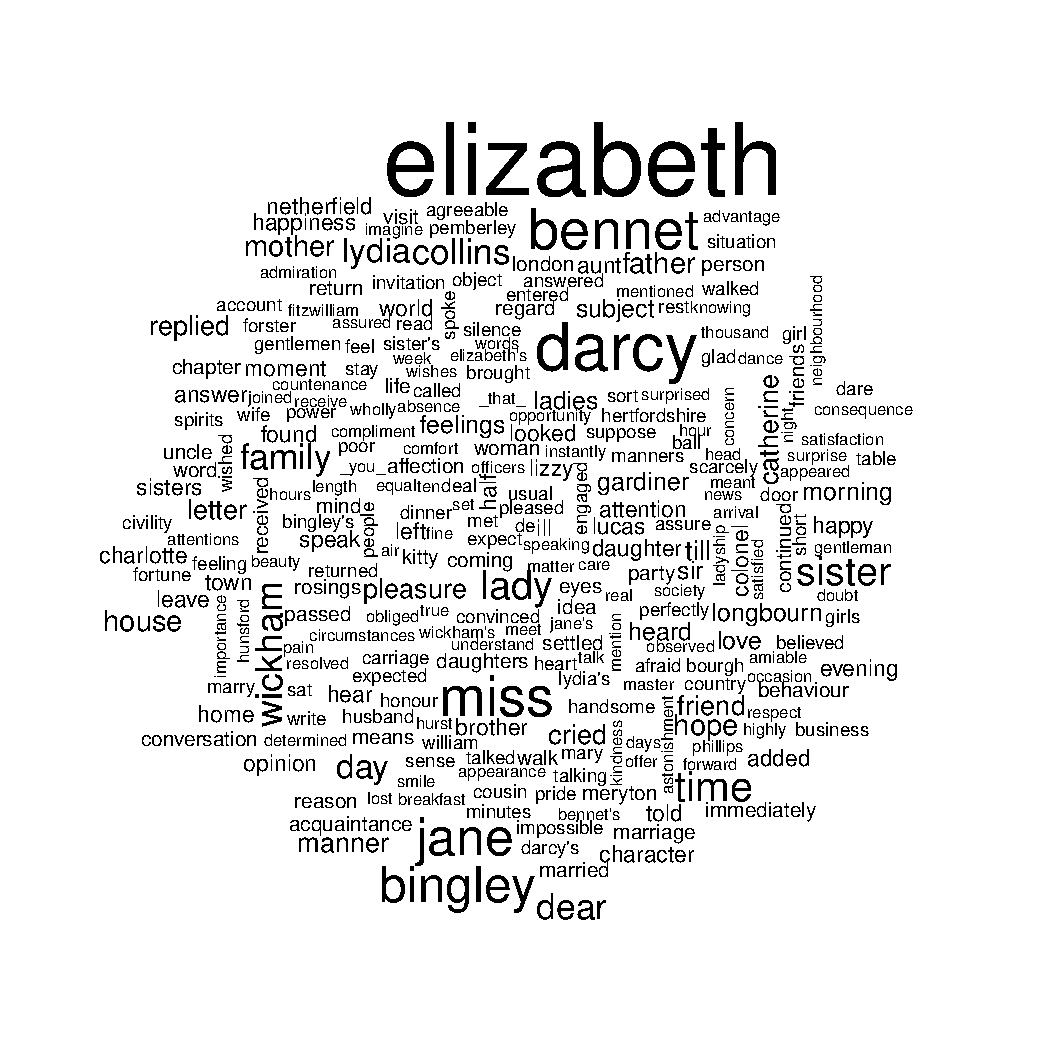
\includegraphics[width=\maxwidth]{figure/unnamed-chunk-8-1} 

\end{knitrout}

\bibliographystyle{apa}
\bibliography{article}
\nocite{*}

\end{document}
